\section*{Atomicity-Violation Bugs (Non-Deadlock)}
\begin{minipage}{0.5\linewidth}
\begin{lstlisting}[language=c]
Thread 1::
if (thd->proc_info) {
  fputs(thd->proc_info, ...);
}       // ^ may deref NULL
Thread 2::
thd->proc_info = NULL;
\end{lstlisting}
\end{minipage}
\begin{minipage}{0.5\linewidth}
  \flushleft
  \begin{itemize}
  \item two $T$s access \texttt{proc\_info} in \texttt{thd}
  \item if $T_1$ checked but interrupted by $T_2$ before calling \texttt{fputs}
  \item $T_2$ sets pointer to \texttt{NULL}
  \item $T_1$ resumes and deref \texttt{NULL} ptr, BOM!
  \end{itemize}
\end{minipage}
\begin{itemize}
\item the code has an atomicity assumption about the check for non-NULL of \texttt{proc\_info} and the usage of \texttt{proc\_info} in the \texttt{fputs()} call
\item when the assumption is incorrect, the code will not work as desired
\end{itemize}
\begin{lstlisting}[language=c]
pthread_mutex_t pinfo_lock = PTHREAD_MUTEX_INITIALIZER;
\end{lstlisting}
\begin{minipage}{0.5\linewidth}
\begin{lstlisting}[language=c]
Thread 1::
pthread_mutex_lock(&pinfo_lock);
if (thd->proc_info) {
   fputs(thd->proc_info, ...);
}
pthread_mutex_unlock(&pinfo_lock);
\end{lstlisting}
\end{minipage}
\begin{minipage}{0.5\linewidth}
\begin{lstlisting}[language=c,xleftmargin=4pt]
// lock the critical section
Thread 2::
pthread_mutex_lock(&pinfo_lock);
thd->proc_info = NULL;
pthread_mutex_unlock(&pinfo_lock);
thd->proc_info = NULL;
\end{lstlisting}
\end{minipage}
\section*{Order-Violation Bugs (Non-Deadlock)}
\begin{minipage}{0.5\linewidth}
\begin{lstlisting}[language=c]
Thread 1::
void init() {
 mThread = PR_CreateThd(mMain,...);
}
\end{lstlisting}
\end{minipage}
\begin{minipage}{0.5\linewidth}
\begin{lstlisting}[language=c,xleftmargin=4pt]
Thread 2::
void mMain(...) {
  mState = mThread->State;
}// may deref NULL ^
\end{lstlisting}
\end{minipage}
\begin{itemize}
\item $T_2$ assumes \texttt{mThread} already init (non-NULL) while accessing it
\item yet if $T_2$ runs before $T_1$ $\to$ \texttt{mThread == NULL}, BOM! deref NULL ptr
\item to fix this type of bug $\to$ use \mo{cond var}/\mo{semaphore} to enforce ordering
\end{itemize}
\begin{lstlisting}[language=c]
pthread_mutex_t mtLock = PTHREAD_MUTEX_INITIALIZER; // lock
pthread_cond_t  mtCond = PTHREAD_COND_INITIALIZER;  // cond var
int mtInit = 0; // state variable
Thread 1::
void init() {
  // other work ...
  mThread = PR_CreateThread(mMain, ...);
  // signal that the thread has been created...
  pthread_mutex_lock(&mtLock);
  mtInit = 1; // set state
  pthread_cond_signal(&mtCond);
  pthread_mutex_unlock(&mtLock);
  // other work ...
}
Thread 2::
void mMain(...) {
  // other work ...
  // wait for the thread to be initialized...
  pthread_mutex_lock(&mtLock);
  while (mtInit == 0)
    pthread_cond_wait(&mtCond, &mtLock); // wait for state to be set
  pthread_mutex_unlock(&mtLock);
  mState = mThread->State;
  // other work ...
}
\end{lstlisting}
\begin{minipage}{0.5\linewidth}
  \section*{Deadlock}
\begin{lstlisting}[language=c,frame=lines]
Thread 1::
pthread_mutex_lock(L1);
pthread_mutex_lock(L2);
Thread 2::
pthread_mutex_lock(L1);
pthread_mutex_lock(L2);
\end{lstlisting}
  \flushleft
  \begin{itemize}
  \item deadlock \emph{may} occur when
  \item $T_1$ holds \texttt{L1}, waiting for \texttt{L2}
  \item $T_2$ holds \texttt{L2}, waiting for \texttt{L1}
  \end{itemize}
\end{minipage}
\begin{minipage}{0.5\linewidth}
  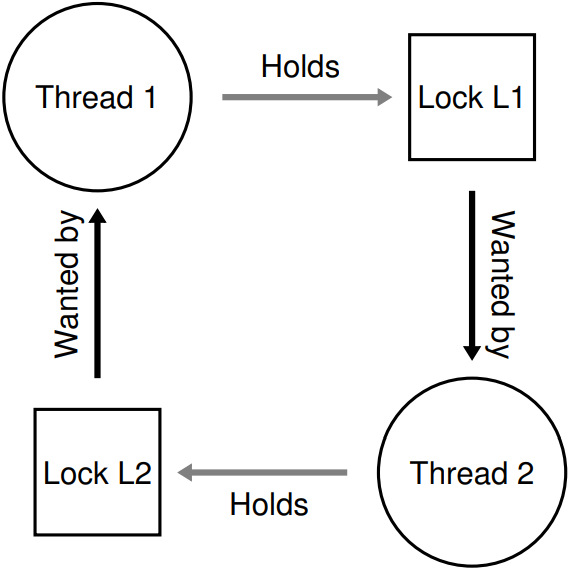
\includegraphics[width=\linewidth,height=3.6cm]{imgs/deadlocks1}
\end{minipage}
\section*{Reasons for Deadlock}
\begin{enumerate}
\item circular dependencies between threads and resources, such that none of the threads can acquire the required resources to make progress
\item encapsulation: modularity does not mesh well with locking
\end{enumerate}
\section*{4 must-hold conds for a deadlock to occur (any unmet, no deadlock)}
\begin{itemize}
\item \textbf{Mutual exclusion} Threads claim exclusive control of resources that they require (e.g. a thread grabs a lock)
\item \textbf{Hold-and-wait} Threads hold resources they already acquired (e.g. locks) while waiting for extra resources (locks they wish to acquire)
\item \textbf{No preemption} can't forcibly rm resources from $T$s holding them
\item \textbf{Circular wait} a circular chain of $T$s such that each $T$ holds one or more resources (e.g. locks) being requested by the next $T$ in the chain
\end{itemize}
\section*{Prevent circular wait $\to$ total/partial ordering on lock acquisition}
\begin{itemize}
\item if \emph{only} 2 locks (\texttt{L1},\texttt{L2}), strict ordering: always acquire \texttt{L1} before \texttt{L2}
\item lock acquisition must respect the partial ordering (reflexive, transitive, anti-symmetric) $\to$ guarantee no circularity
\end{itemize}
\begin{minipage}{0.5\linewidth}
\begin{lstlisting}[language=c,xleftmargin=2pt]
// fn need to grabs two locks
do sth(mutex t *m1, mutex t *m2)
\end{lstlisting}
  \begin{itemize}
  \item if always grabs \texttt{m1} before \texttt{m2} (or \texttt{m2} before \texttt{m1}) $\to$ may deadlock
  \item $\because T_1$ calls \texttt{do\_sth(m1, m2)} while $T_2$ calls \texttt{do\_sth(m2, m1)} $\to$ deadlock
  \item $T_1$ waits for \texttt{m2}; $T_2$ waits for \texttt{m1}
  \item fix: enforce ordering by lock addr
  \end{itemize}
\end{minipage}
\begin{minipage}{0.5\linewidth}
\begin{lstlisting}[language=c,xleftmargin=4pt,framextopmargin=1pt]
// grab in high-to-low addr order
if (m1 > m2) {
  pthread_mutex_lock(m1);
  pthread_mutex_lock(m2);
} else {
  pthread_mutex_lock(m2);
  pthread_mutex_lock(m1);
}
// assume m1 != m2 (not same lock)
\end{lstlisting}
\end{minipage}
\section*{Prevent hold-and-wait $\to$ acquire all locks at once, atomically}
\begin{minipage}{0.75\linewidth}
\begin{lstlisting}[language=c,xleftmargin=2pt]
pthread_mutex_lock(prevention); // begin acquisition
pthread_mutex_lock(L1);
pthread_mutex_lock(L2);
...
pthread_mutex_unlock(prevention); // end
\end{lstlisting}
\end{minipage}
\begin{minipage}{0.3\linewidth}
  \flushleft
  \begin{itemize}
  \item \mb{must} first grab \texttt{prevention} lock
  \item ensure no untimely $T$ switch can occurs $\to$ avoid deadlock
  \end{itemize}
\end{minipage}
\begin{itemize}
\item Ok for $T$ to acquire \texttt{L1}$\cdots$\texttt{L2} in any order $\because$ it already holding \texttt{L}$_\text{prevention}$
\item must know exactly which locks must be held and acquire ahead of time
\item concurrency $\downarrow$ $\because$ must acquire all locks at once even when not need to
\end{itemize}
\begin{minipage}{0.56\linewidth}
\section*{Add Preemption: imperfect, working}
\begin{lstlisting}[language=c,xleftmargin=2pt]
top:
  pthread_mutex_lock(L1);
  if (pthread_mutex_trylock(L2) != 0) {
    pthread_mutex_unlock(L1);
    goto top;
  }
\end{lstlisting}
\end{minipage}
\begin{minipage}{0.44\linewidth}
  \flushleft
  \begin{itemize}
  \item deadlock-free, ordering-robust lock acquisition protocol:
  \item try to grab lock if available $\to$ success
  \item if lock held by other $\to$ error; try again later
  \end{itemize}
\end{minipage}
\begin{itemize}
\item $T_{\text{other}}$ could follow same protocol but grab lock in order of \texttt{L2} then \texttt{L1}
\item this leads to \mo{livelock}: both systems running through this code sequence repeatedly (thus not a deadlock), but progress not being made
\item add a random delay before looping back and trying over again $\to$ decreasing the odds of repeated interference among competing threads
\item[1.] if \texttt{L1} gets dropped in some routine, go-back $\to$ more complex
\item[2.] if along \texttt{L1}, extra mem also acquired, must ensure to release mem too
\item[3.] \emph{not} really \emph{add} preemption, but just preempt its own lock ownership
\end{itemize}
\section*{Prevent Mutual Exclusion (lock-free data struct + hardware help)}
\begin{minipage}{0.5\linewidth}
\begin{lstlisting}[language=c]
int CompAndSwap(
  int *addr, int expected, int new
) {
  if (*addr == expected) {
    *addr = new;
    return 1; // success
  }
  return 0; // failure
} // atomic ix provided by hardware
\end{lstlisting}
\end{minipage}
\begin{minipage}{0.5\linewidth}
\begin{lstlisting}[language=c,xleftmargin=2pt]
void AtomicIncrement(
  int *val, int amt
) {
  do {
    int old = *val;
  } while (
  CompAndSwap(val, old, old + amt)
  == 0); // if val == old, inc old
} // else keep trying
\end{lstlisting}
\end{minipage}
livelock still possible; robust solution will be more complex than above\newline
\begin{minipage}{0.55\linewidth}
\section*{list insertion example}
\begin{lstlisting}[language=c,frame=none,xleftmargin=-6pt]
// thread-unsafe: race condition
void insert(int value) {
  node_t *n = malloc(sizeof(node_t));
  assert(n != NULL);
  n->value = value;
  n->next = head;
  head = n;
}
\end{lstlisting}
\end{minipage}
\begin{minipage}{0.5\linewidth}
\begin{lstlisting}[language=c,frame=none,xleftmargin=-18pt]
void insert(int value) {
  node_t *n = malloc(sizeof(node_t));
  assert(n != NULL);
  n->value = value;
  pthread_mutex_lock(listlock);
  n->next = head;
  head = n;
  pthread_mutex_unlock(listlock);
} // lock critical section
\end{lstlisting}
\end{minipage}
\begin{minipage}{0.68\linewidth}
\begin{lstlisting}[language=c]
void insert(int value) {
  node_t *n = malloc(sizeof(node_t));
  assert(n != NULL);
  n->value = value;
  do {
    n->next = head;
  } while (CompAndSwap(&head, n->next, n) == 0);
} // retry again with new head by other thread
\end{lstlisting}
\end{minipage}
\begin{minipage}{.32\linewidth}
  \flushleft
  \begin{itemize}
  \item point \texttt{next} to curr head and try to make the node new head
  \item this will fail if some other $T$ successfully swapped in a new head in meanwhile
  \item then try again
  \end{itemize}
\end{minipage}
\section*{Deadlock Avoidance via Scheduling}
\begin{minipage}{.4\linewidth}
  \begin{tabular}[ht]{lllll}
    Lock        & \texttt{T1} & \texttt{T2} & \texttt{T3} & \texttt{T4} \\
    \texttt{L1} & yes & yes & \mr{no} & no \\
    \texttt{L2} & yes & yes & yes & no \\
  \end{tabular}
\end{minipage}
\begin{minipage}{.6\linewidth}
  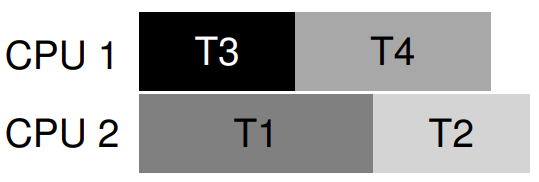
\includegraphics[width=.9\linewidth,height=1.8cm]{imgs/threadsdeadlock2}
\end{minipage}
\begin{itemize}
\item A smart scheduler could ensure T1 and T2 are not run at the same time $\to$ no deadlock could ever arise
\item  it is OK for (T3 and T1) or (T3 and T2) to overlap. Even
though T3 grabs lock \texttt{L2}, it can never cause a deadlock by running concurrently with other threads because it only grabs one lock
\end{itemize}
\begin{minipage}{.4\linewidth}
  \begin{tabular}[ht]{lllll}
    Lock        & \texttt{T1} & \texttt{T2} & \texttt{T3} & \texttt{T4} \\
    \texttt{L1} & yes & yes & \mr{yes} & no \\
    \texttt{L2} & yes & yes & yes & no \\
  \end{tabular}
\end{minipage}
\begin{minipage}{.6\linewidth}
  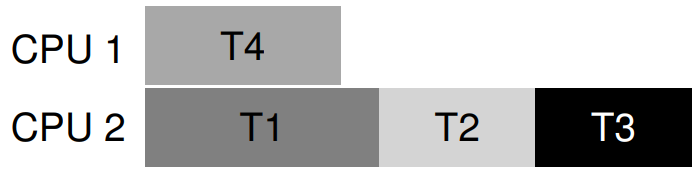
\includegraphics[width=\linewidth,height=1.8cm]{imgs/threadsdeadlock3}
\end{minipage}
\begin{itemize}
\item T1, T2, and T3 all need to grab both locks \texttt{L1} and \texttt{L2} at some point
\item static scheduling leads to conservative approach: T1, T2, T3 all run on same processor: $\to T_{\text{total-completion-time}} \uparrow$ considerably
\item deadlock avoidance: not a widely-used general-purpose solution
\end{itemize}
\section*{Detect and Recover}
\begin{itemize}
\item allow deadlocks to occasionally occur $\to$ reboot once detected it
\item this non-solution is indeed pragmatic if deadlocks are rare
\item Many DBMS employ deadlock detection and recovery techniques
\item deadlock detector runs periodically, building a resource graph and checking for cycles; when there's a cycle (deadlock), sys needs reboot
\end{itemize}
\begin{tcolorbox}[left=0mm, top=1mm, right=0mm, rightlower=0mm, bottom=1mm,
  title=USE ATOMIC OPERATIONS,
  halign title=center]
  The idea behind making a series of actions \textbf{atomic}: ``all or nothing''. It should either appear as if all of the actions you wish to group together occurred, or that none of them occurred, with no in-between state visible. Sometimes, the grouping of many actions into a single atomic action is called a \textbf{transaction}
\end{tcolorbox}
\begin{tcolorbox}[left=0mm, top=1mm, right=0mm, rightlower=0mm, bottom=1mm,
  title= DON'T ALWAYS DO IT PERFECTLY (TOM WEST'S LAW),
  halign title=center]
  ``Not everything worth doing is worth doing well'': If a bad thing happens rarely, certainly one should not spend much effort to prevent it, \emph{particularly if} the cost of the bad things is small. With pressing deadlines and other real-world concerns, one will always have to decide which aspects of a system to build well and which to put aside
\end{tcolorbox}
